\documentclass{standalone}
\usepackage{tikz}
\usepackage{ctex,siunitx}
\usepackage{tkz-euclide}
\usepackage{amsmath}
\usetikzlibrary{patterns, calc}
\usetikzlibrary {decorations.pathmorphing, decorations.pathreplacing, decorations.shapes,}
\begin{document}
\small
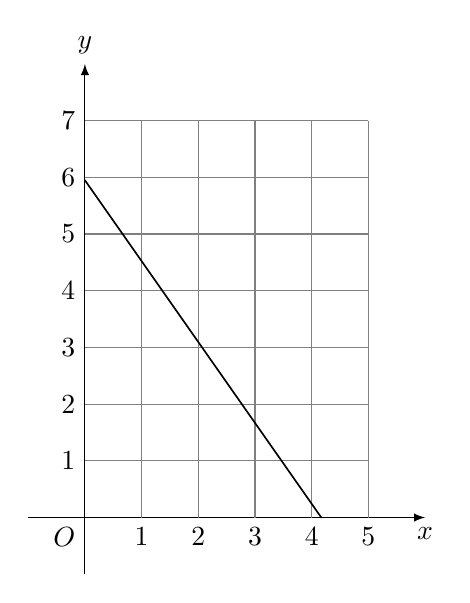
\begin{tikzpicture}[>=latex,scale=0.72]
  \draw[thin,->](-1,0)--(6,0)node[below]{$x$};
  \draw[thin,->](0,-1)--(0,8)node[above]{$y$};
  \tkzDefPoints{0/0/O,0/5.95/M,4.17/0/N}
  \foreach \x in {1,...,5}
  {
    \draw[thin,gray](\x,7)--++(0,-7)node[below,text=black]{$\x$};
  }
  \foreach \x in {1,...,7}
  {
    \draw[thin,gray](5,\x)--++(-5,0)node [left,text=black]{$\x$};
  }
  \tkzDrawSegments[semithick](N,M)
  \tkzLabelPoints[below left](O)
\end{tikzpicture}
\end{document}